\documentclass[xcolor=dvipsnames,10pt]{beamer}
% ********** Styl prezentacji **********
\mode<presentation>
{
%\usetheme{Frankfurt}
%\usetheme{Copenhagen}
\usetheme{Madrid}
 %\usetheme{lankton-keynote}
 %Copenhagen
}
%\usepackage{amsmath}
%\usepackage{amsthm}
%\usepackage{amsfonts}
\usepackage{color}
%\usepackage{listings}
%\lstset{language=C++}
%\usepackage{lscape} 
%\usepackage{float}
%\usepackage{graphicx}
\usepackage{caption}
\usepackage{subcaption}
%\usepackage{multimedia}
% common reference commands
\renewcommand{\Re}{\textrm{Re}}
\newcommand{\Pe}{\textrm{P\'e}}
\renewcommand{\Pr}{\textrm{Pr}}
\newcommand{\eqt}[1]{Eq.~(\ref{#1})}                     % equation
\newcommand{\fig}[1]{Fig.~\ref{#1}}                      % figure
\newcommand{\tbl}[1]{Table~\ref{#1}}                     % table
%\usepackage{movie15}
%\usepackage{hyperref}
%\usepackage{multimedia}
\usepackage[]{media9}
%\usepackage{filecontents,hyperref,listings}
\renewcommand{\div}{\boldsymbol{\nabla}\! \cdot \!}
\newcommand{\grad}{\boldsymbol{\nabla}}
\newcommand{\divv}[1]{\boldsymbol{\nabla}^{#1}\! \cdot \!}
\newcommand{\gradd}[1]{\vec{\nabla}^{#1}}
\newcommand{\mbold}[1]{\boldsymbol#1}
%
%\setbeamertemplate{footline}[frame number]
%\title{Extension of the entropy viscosity method to low Mach regime and the seven equations model.}
%\title{Extension of the entropy viscosity method to low Mach regime and the seven equations model.}
%\author{Marc-Olivier Delchini}
%
\begin{document}
%
%\begin{frame}
%\maketitle
%\end{frame}
\begin{frame}
\begin{center}
Extension of the entropy viscosity method to the low Mach multi-D Euler equations and the seven-equation model.
\begin{center}
by \\
Marc-Olivier Delchini
\end{center}
\today \\

Co-chairs: J. Ragusa\footnote{Nuclear Engineering Department, Texas A\&M University.} and J.L. Guermond\footnote{Department of Mathematics, Texas A\&M University.}. \\
Committee members: J. Morel\footnotemark[1], Y. Hassan\footnotemark[1] and R. Berry\footnote{Idaho National Laboratory.}.
\end{center}
\end{frame}
%
\begin{frame}
	\frametitle{Outline:}
	\tableofcontents
\end{frame}
%************************************************
\section{Introduction}
\begin{frame}
introduction $\to$ hyperbolic system of equations and real life
\end{frame}
%************************************************
\begin{frame}{Mathematical propoerties}
Let us consider a hyperbolic conservation law of the form:
\begin{equation} \partial_t \mbold U + \div \mbold F \left( \mbold U \right) = \mbold 0  \nonumber \text{ (strong form)}\end{equation} 
\begin{itemize}
\item wave-dominated problem $\to$ eigenvalues.
\item known to form shocks even with smooth initial conditions: characteristic equation and variable (REFS)
\item require a numerical stabilization method to resolve shocks: approximate Riemann solver, artificial dissipative method, flux-limiting method, $\dots$
\item uniqueness of the weak solution is ensured by an entropy condition: the associated entropy equation satisfies an inequality and is peaked in the shock region.
\begin{equation}
\partial_t S\left( \mbold U\right) + \grad \Phi \left( \mbold U \right) \geq 0  \nonumber
\end{equation}
\end{itemize}
\end{frame}
%************************************************
\begin{frame}{The general idea behind the entropy viscosity method}
\emph{It is an artificial dissipation method with smart viscosity coefficient capable of tracking the shock so that dissipation is only added into the shock region.}
\begin{block}{}
\begin{itemize}
\setlength{\itemsep}{10pt}
\item it requires a viscous regularization: the dissipative terms are consistent with the entropy inequality.
\item each viscosity coefficient is function of a high-order viscosity coefficient and an upper bound called first-order viscosity coefficient.
\item the high-order viscosity coefficient is defined proportional to the entropy residual.
\item the first-order viscosity coefficient is function of the local maximum eigenvalue.
\item also accounts for the inter element jumps $\to$ make the definition of the viscosity coefficients also sensitive to all discontinuities. 
\end{itemize}
\end{block}
\end{frame}
%************************************************
\begin{frame}{The Multiphysics Object-Oriented Simulations Environment (MOOSE)}
\begin{block}{}
\begin{itemize}
\setlength{\itemsep}{10pt}
\item Explicit and implicit temporal integrators (first and second-order accuracy)
\item Continuous and Discontinuous Galerkin Finite Element Method
\item Mesh adaptivity, time step adaptivity
\item Support parallel runs
\item Buildt on PETSc and Libmesh
\item For implicit solve, requires a preconditioner $\to$ either FDP or hard-coded preconditioner
\item C++ language, opened source
\end{itemize}
\end{block}
\begin{block}{}
All numerical solutions were run with BDF2 and linear test functions $\to$ second-order accuracy in time and space.
\end{block}
\end{frame}
%************************************************
\begin{frame}{A simple example of application of the EVM: the $1$-D Burger's equation}
\begin{block}{The $1$-D Burger's equation with its viscous regularization}
\begin{equation}
\partial_t u(x,t) + \partial_x \left( \frac{u(x,t)^2}{2} \right) = \textcolor{blue}{\partial_x \left( \mu \left(x,t \right) \partial_x u(x,t) \right)} \nonumber
\end{equation}
\end{block}
\begin{block}{Definition of the local viscosity coefficient $\mu(x,t)$}
\begin{align}
&\mu(x,t) = \min \left( \mu_e(x,t), \mu_{max}(x,t) \right) \nonumber \\
&\mu_{max} (x,t) = \frac{h}{2} | u(x,t) | \nonumber \\
&\mu_e(x,t) = h^2 \frac{\max \left( R(x,t), J \right)}{|| \eta(u) - \bar{\eta}(t) ||_\infty} \nonumber \\
& \text{Entropy residual: }R(x,t) = \partial_t \eta(u) + \partial_x \Phi(u) \leq 0 \text{ with } \eta(u) = u^2 / 2 \nonumber \\
&\text{Jump: } J = [[ \partial_x \Phi(u) ]] \nonumber
\end{align}
\end{block}
\end{frame}
%************************************************
\begin{frame}{$1$-D numerical results (100 cells and CFL $=1$}
\begin{figure}[H]
        \centering
        \begin{subfigure}[b]{0.37\textwidth}
                \centering
                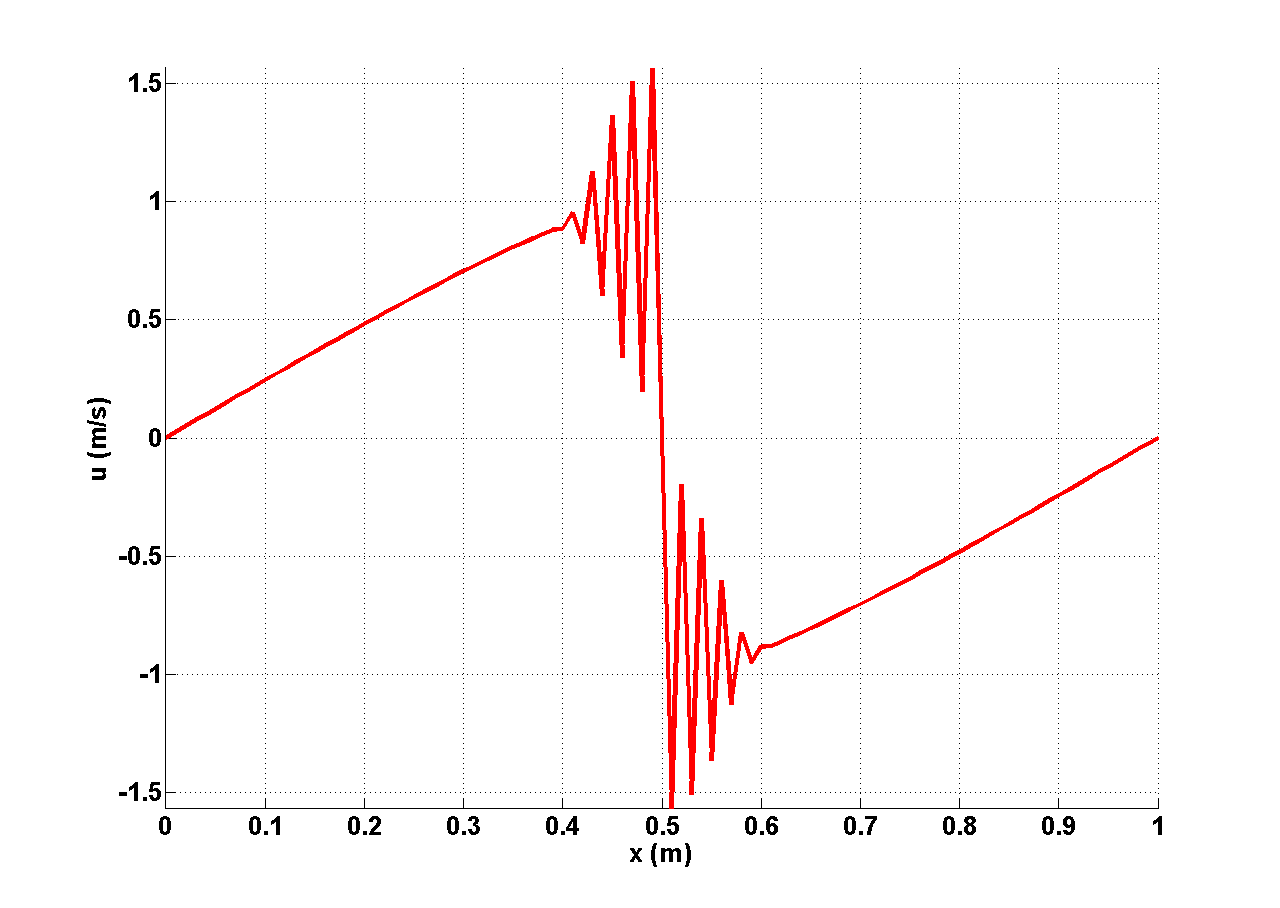
\includegraphics[width=\textwidth]{../figures/1D_sol_free.png}
                \caption{Without stabilization.}
                \label{fig:1d_burger_free}
        \end{subfigure}%
        \begin{subfigure}[b]{0.37\textwidth}
                \centering
                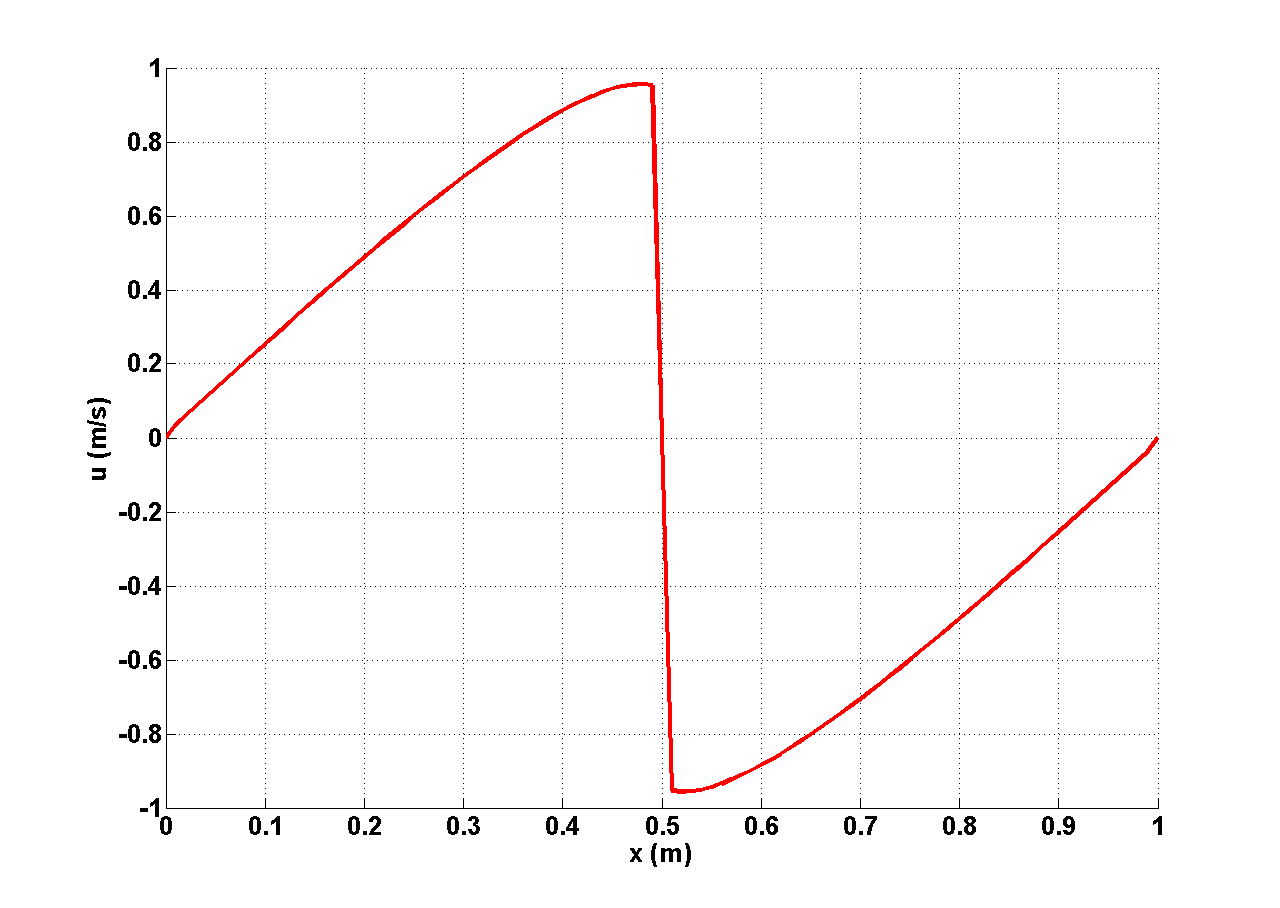
\includegraphics[width=\textwidth]{../figures/1D_sol_fo.png}
                \caption{With first-order viscosity.}
                \label{fig:1d_burger_fo}
        \end{subfigure}
        
        \begin{subfigure}[b]{0.37\textwidth}
                \centering
                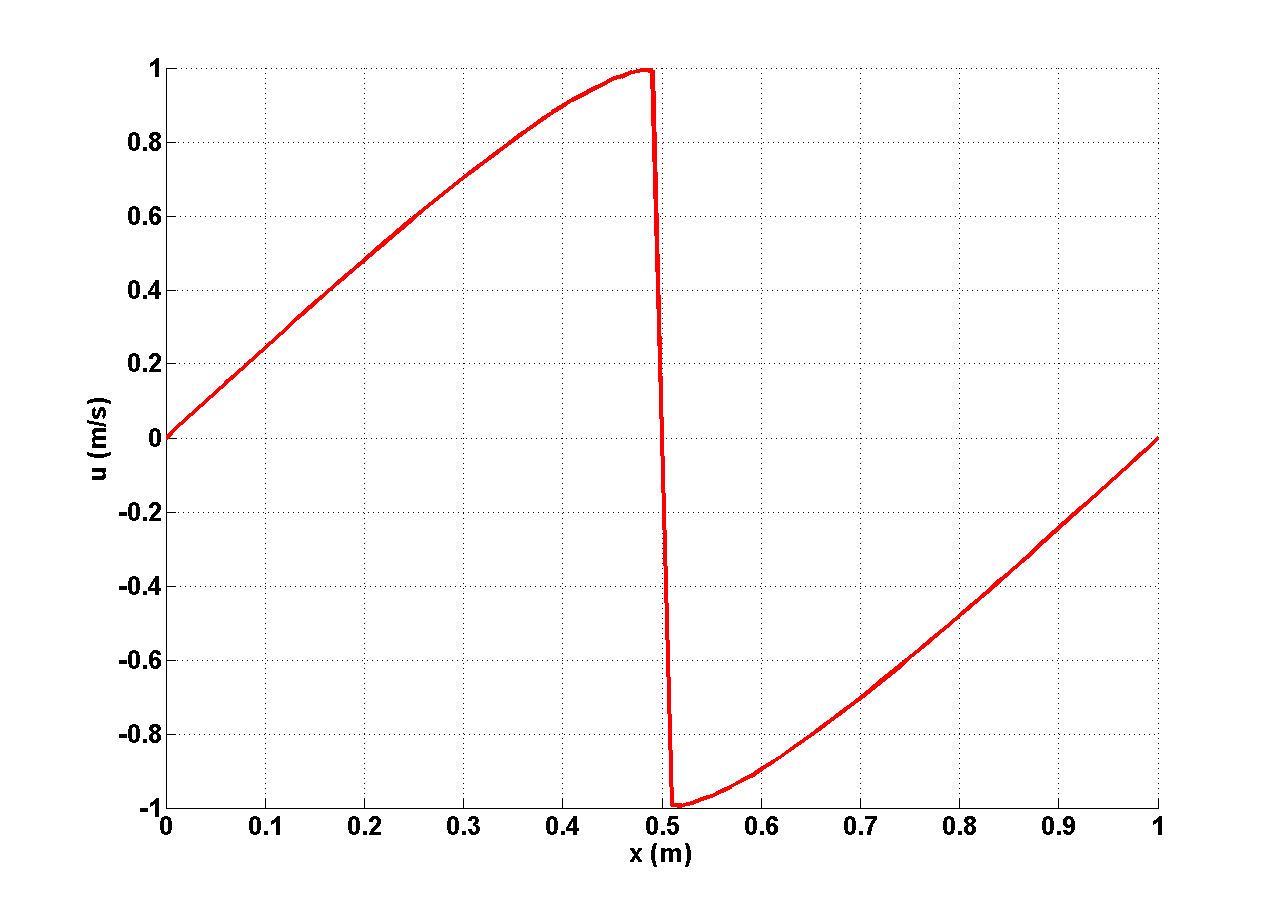
\includegraphics[width=\textwidth]{../figures/1D_sol_ev.png}
                \caption{With the EVM.}
                \label{fig:1d_burger_ev}
        \end{subfigure}
        \begin{subfigure}[b]{0.37\textwidth}
                \centering
                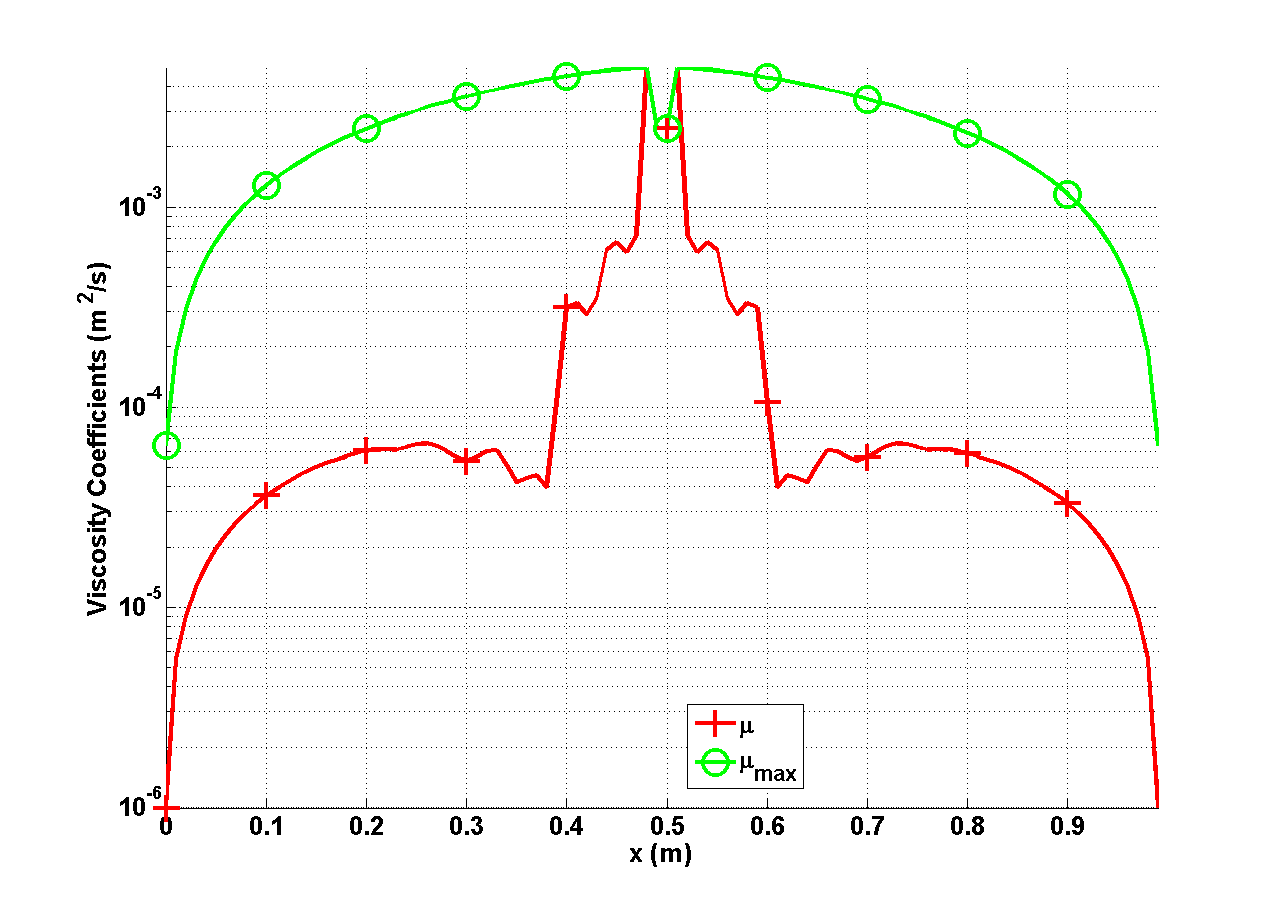
\includegraphics[width=\textwidth]{../figures/1D_visc.png}
                \caption{Viscosity coefficient profiles.}
                \label{fig:1d_burger_visc}
        \end{subfigure}
\end{figure}
\end{frame}
%************************************************
\section{The multi-D Euler equations with variable area}
\begin{frame}
\begin{center}
The multi-D Euler equations with variable area
\end{center}
\end{frame}
%************************************************
\begin{frame}
\begin{block}{Numerical methods for continuous and discontinuous schemes}
\begin{itemize}
\setlength{\itemsep}{10pt}
\item multi-wave problem, can develop shock waves and other types of discontinuities. 
\item Numerical methods for both continuous and discontinuous schemes: approximate Riemann solvers (HLL, HLLC, Roe scheme, $\cdots$), flux limiters
, Lapidus viscosity, Pressure-based viscosity, SUPG, C-method, Entropy Viscosity Method (EVM). 
\item Numerical method can be ill-scaled in the low-Mach limit, yielding the wrong incompressible system $\to$ use of a Mach-based preconditioner for the dissipative terms to obtain the correct behavior in the low Mach limit.
\item Low-Mach steady-state solution: time-dependent term preconditioner to accelerate the convergence of the solution to the steady-state (Turkel) when using an explicit scheme $\to$ the transient is no longer accurate. \emph{Implicit solvers do not have this issue}. 
\end{itemize}
\end{block}
\end{frame}
%************************************************
\begin{frame}
\begin{block}{}
\begin{itemize}
\setlength{\itemsep}{10pt}
\item The isentropic compressible multi-D Euler equations degenerate into an incompressible system in the low-Mach asymptotic limit.
\begin{align}
&\partial_t \rho + \vec{u} \cdot \grad \rho = 0 \nonumber \\
&\partial_t \vec{u} + \vec{u}\text{ } \div \vec{u} + \frac{1}{\rho}\grad P = 0 \nonumber \\
&P( \vec{r},t) = P_0(t) + M^2 P_2(\vec{r},t)\nonumber
\end{align}
$\to$ no energy equation since the flow is assumed isentropic \\
$\to$ pressure fluctuations of the order of the Mach number square
\end{itemize}
\end{block}
\end{frame}
%************************************************
\begin{frame}
\begin{block}{The multi-D Euler equations with variable area}
\begin{align}
&\text{Mass conservation} \nonumber \\
&\partial_t ( \rho A ) + \div \left( \rho A \vec{u} \right) = 0 \nonumber \\
&\text{Momentum conservation} \nonumber \\
&\partial_t ( \rho \vec{u} A ) + \div \left( \rho A \vec{u} \otimes \vec{u} + P \mathbb{I} \right) = P \grad A \nonumber \\
&\text{Energy conservation} \nonumber \\
&\partial_t ( \rho E A ) + \div \left[ \vec{u} \left( \rho E + P \right) A \right] = 0 \nonumber \\
&\text{Equation of state} \nonumber \\
& P = eos \left( \rho, e \right) \nonumber 
\end{align}
\end{block}
Multi-wave problem: $\lambda_1 = \vec{u} \cdot \vec{n} - c $, $\lambda_2 = \vec{u} \cdot \vec{n} + c $ and $\lambda_{2, \dots, 2+D} = \vec{u} \cdot \vec{n}$. \\
The area $A$ is only a function of space.
\end{frame}
%************************************************
\begin{frame}
\emph{Objectives: extend the EVM to low-Mach flows while maintaining its capabilities of solving for transonic and supersonic flows, and use an implicit solver.}
\begin{block}{How to do it?}
\begin{enumerate}
\setlength{\itemsep}{10pt}
\item derive a viscous regularization for the multi-D Euler equations (already done).
\item work with the non-dimensionalized version of the multi-D Euler equations in order to understand how the different terms scale $\to$ will define non-dimensionalized numbers (Mach number, numerical Reynolds number, $\dots$)
\item derive a definition for the viscosity coefficients that ensures well-scaled dissipative terms for a wide range of Mach numbers $\to$ will consider two cases: isentropic and non-isentropic.
\end{enumerate}
\end{block}
\end{frame}
%************************************************
\begin{frame}{A viscous regularization for the multi-D Euler equations with variable area}
\begin{align}
&\text{Mass conservation} \nonumber \\
&\partial_t ( \rho A ) + \div \left( \rho A \vec{u} \right) = \textcolor{blue}{\div \vec{f}} \nonumber \\
&\text{Momentum conservation} \nonumber \\
&\partial_t ( \rho \vec{u} A ) + \div \left( \rho A \vec{u} \otimes \vec{u} + P \mathbb{I} \right) = P \grad A + \textcolor{blue}{\div \left( \mathbb{F}(\vec{u}) + \vec{u} \otimes \vec{f} \right)} \nonumber \\
&\text{Energy conservation} \nonumber \\
&\partial_t ( \rho E A ) + \div \left[ \vec{u} \left( \rho E + P \right) A \right] = \textcolor{blue}{\div \left( \vec{h} + \vec{u}\cdot \mathbb{F}(\vec{u}) + \frac{|| \vec{u} ||^2}{2} f \right)} \nonumber \\
&\text{Dissipative terms} \nonumber \\
& \textcolor{blue}{\vec{f} = A \kappa \grad \rho \text{, } \vec{h} = A \kappa \grad ( \rho e) } \nonumber
\text{ and } \textcolor{blue}{\mathbb{F}(\vec{u}) = A \mu \grad^s \vec{u}} \text{ or } \textcolor{blue}{\mathbb{F}(\vec{u}) = A \mu \grad \vec{u}}
\end{align}
$\to$ two positive viscosity coefficients $\mu$ and $\kappa$. Requires a concave physical entropy $s(\rho,e)$.
\end{frame}
%************************************************
\begin{frame}{Non-dimensionalized multi-D Euler equation}
We define some reference variables denoted by subscript $\infty$:
\begin{multline}
\label{eq:norm_param}
\rho^*   = \frac{\rho}{\rho_\infty}           ,\
u^*      = \frac{u}{u_\infty}                 ,\
P^*      = \frac{P}{\rho_\infty c^2_\infty}   ,\
E^*      = \frac{E}{c^2_\infty }              ,\\
x^* = \frac{x}{L_\infty}                      ,\
t^* = \frac{t}{L_\infty / u_\infty}           ,\ 
\textcolor{blue}{\mu^*    = \frac{\mu}{\mu_\infty}}             ,\
\textcolor{blue}{\kappa^* = \frac{\kappa}{\kappa_\infty}}     \nonumber
\end{multline}
We also define the following reference numbers:
\begin{align}
&\text{Mach number: }M_\infty = \frac{u_\infty}{c_\infty}, \nonumber\\
&\text{Numerical Reynolds number: }\Re_\infty = \frac{u_\infty L_\infty}{\mu_\infty} , \nonumber \\
&\text{Numerical P\'echlet number: }\Pe_\infty = \frac{u_\infty L_\infty}{\kappa_\infty} , \nonumber \\
&\text{Numerical Prandlt number: }\Pr_\infty = \Pe_\infty / \Re_\infty \nonumber \nonumber
\end{align}
\end{frame}
%************************************************
\begin{frame}{Non-dimensionalized multi-D Euler equation}
\begin{subequations} 
\label{eq:Euler_eq2}
%
\begin{equation}
\partial_{t^*} \rho^*+ \divv{*}  \left(  \rho^* \vec{u}^*  \right) = \textcolor{blue}{\frac{1}{\Pe_\infty} \divv{*}  ( \kappa^* \gradd{*} \rho^* )} \nonumber
\end{equation}
%
\begin{align}
\partial_{t^*} \left( \rho^* \vec{u}^* \right) 
+ \divv{*} \left( \rho^* \vec{u}^*\otimes \vec{u}^* \right) 
+ \textcolor{magenta}{\frac{1}{M_\infty^2}\gradd{*}  P^*}  
&= 
\textcolor{blue}{\frac{1}{\Re_\infty} \divv{*} \left( \rho^* \mu^* \gradd{s,*} \vec{u}^* \right)}  \nonumber\\
&+
\textcolor{blue}{\frac{1}{\Pe_\infty} \divv{*} \left(\vec{u}^*\otimes \kappa^* \gradd{*}  \rho^* \right)} \nonumber
\end{align}
%
\begin{align}
\partial_{t^*} \left( \rho^* E^* \right) 
+ \divv{*}  \left[ \vec{u}^* \left( \rho^* E^* + P^* \right) \right] 
&=
\textcolor{blue}{\frac{1}{\Pe_\infty} \divv{*}  \left( \kappa^*  \gradd{*} (\rho^* e^*) \right)} \nonumber  \\
+
\textcolor{blue}{\frac{M_\infty^2}{\Re_\infty} \divv{*}  \left( \vec{u}^* \rho^* \mu^* \gradd{s,*} \vec{u}^* \right)}
&+ 
\textcolor{blue}{\frac{M_\infty^2}{2 \Pe_\infty} \divv{*}  \left(\kappa^* (u^*)^2 \gradd{*} \rho^* \right)} \nonumber
\end{align}
%
\end{subequations}
The above equations are valid for both isentropic and non-isentropic flows and for all Mach numbers.
\end{frame}
%************************************************
\begin{frame}{}

\end{frame}
%************************************************
\end{document}